\documentclass{article}

\usepackage{amsmath}
\usepackage{caption}
\usepackage{fancyhdr}
\usepackage{float}
\usepackage[a4paper, margin=1in]{geometry}
\usepackage{graphicx}
\usepackage{hyperref}
\usepackage{indentfirst}
\usepackage{wrapfig}
\usepackage{xurl}


\linespread{1}


\pagestyle{fancy}
\fancyhead[L]{Book of Specification : \textit{Word search - OCR}}
%\fancyfoot[L]{TriOCR}
\fancyfoot[C]{
    \begin{minipage}{1.5cm}
        \centering
        
\includegraphics[width=1cm]{illustrations/Epita.png}
    \end{minipage}
}
\fancyfoot[R]{\thepage}


\renewcommand{\footrulewidth}{0.1pt}
\renewcommand{\sectionmark}[1]{}
\renewcommand{\subsectionmark}[1]{}
\renewcommand{\contentsname}{}


\title{\textbf{Final Defense Report}\\
\textbf{\textit{Word search - OCR}}}
\date{December 2025}
\author{
    \begin{minipage}[c]{\textwidth}
        \centering
        
\includegraphics[width=5in]{illustrations/Epita.png}
    \end{minipage}
}










\begin{document}

\maketitle

\vfill
\begin{center}
    \textbf{Bidault Quentin}\\
    \textbf{Le Berre Adrien}\\
    \textbf{Lin Jérôme}\\
    \textbf{Class : A1-C1}
\end{center}






\newpage
\thispagestyle{empty}
\addtocounter{page}{-1}
\null
\newpage

\section{Context and objectives}

\section{Functional description}
The system provides tools for creating, managing, and organizing tasks, along with mechanisms for storing and handling user data. It defines how users interact with the application and what features are available to support efficient task management.
\subsection{Task Management}
\section{Technical constraints}
Users gain access to functions allowing creation, modification and deletion of tasks. A title along with status appears within every task entry. Among choices: pending, in progress, completed one serves as the sole status option. Description or priority might appear alongside required elements. Scaling from optional through critical defines how urgency ranks across levels.

Completion of a repeating task triggers creation of a fresh occurrence, guided by an established repetition pattern. Following such completion, the platform produces another version without manual input. Frequencies available for repetition consist of every day, each week, or once per month. This behavior applies only when rules are already defined within settings.

Categories can be created, changed, or removed by users through the system. Following a category removal, linked tasks remain unless specified otherwise. One at a time, adjustments must be made manually for affected tasks. A task might belong to one category, though it may exist independently if needed. Decisions about unlinked tasks rest solely with the user after deletion.

\subsection{Task Organization}
A built-in sorting function helps users arrange tasks by different attributes. Depending on preference, entries appear ordered by name, deadline, urgency, or completion state. One option lets people group items alphabetically through their titles. Another path organizes assignments by when they are due. Priority tags guide arrangement based on importance levels. Status indicators allow viewing progress stages as a sequence.

One way to sort tasks is by their type. A separate screen exists for every group, showing only the items linked to it. Filtering happens automatically when selecting one of these sections. Views are built specifically around each classification. Navigating between them reveals different sets of assignments.

A built-in calendar display will form part of the system. Through this tool, people can see tasks laid out by planned or deadline dates. As a result, managing time becomes more intuitive. The layout supports clearer scheduling decisions across days.

\subsection{Data Management}
Even if closed, the application retains user information between uses. Information about tasks and groupings remains saved on the device, arranged through organized formats like JSON or CSV files.

Also available is the capability to move data in and out of the system, supporting easier handling across environments. Stored items such as tasks and groupings can exit the platform in file form, useful when shifting platforms or saving copies. Every exchange process maintains accuracy, keeping details unchanged during transfers. Consistency within the database remains intact through each operation.


\subsection{User Interface}
A clean desktop interface appears by default, built for straightforward interaction. A panel lines the left edge while the primary workspace fills the center. Navigation lives in that vertical strip, where users move to tasks, category sections, or the calendar through clickable entries. Categories appear automatically in the menu.

A user sees tasks laid out plainly, each marked by name, current state, urgency level, and deadline. To add or adjust an item, a button triggers a pop-up where data is filled or changed. The layout remains clean and focused on readability.

A calendar pane displays scheduled tasks across months, with weekly views available if needed. Navigation feels natural and simplicity stays central throughout the arrangement.

\subsection{Website}
The project's webpage gives a straightforward look at what the app does along with key functions it supports.

A quick glance reveals how the tool organizes tasks, making daily planning easier for visitors who land there. From there, anyone can grab the latest build. Information on how to use core parts appears early so confusion drops fast once someone begins exploring.

\section{Project organization}
\subsection{Task distribution}
\begin{table}[h!]
    \centering
    \begin{tabular}{|l|l|}
        \hline
        \textbf{Task} & \textbf{Responsible}\\
        \hline
        Basic Task Operation & Adrien\\
        \hline
        Task Details & Adrien\\
        \hline
        Task Categories & Quentin\\
        \hline
        Reccurring Task & Quentin\\
        \hline
        Sorting & Quentin\\
        \hline
        Calendar Integration & Jérôme\\
        \hline
        Persistence (Saving) & Jérôme\\
        \hline
        Import/Export & Jérôme\\
        \hline
        GUI & Jérôme\\
        \hline
        Website & Adrien\\
        \hline
    \end{tabular}
\end{table}

\newpage
\subsection{Gantt Diagram}
\begin{figure}[H]
    \centering
    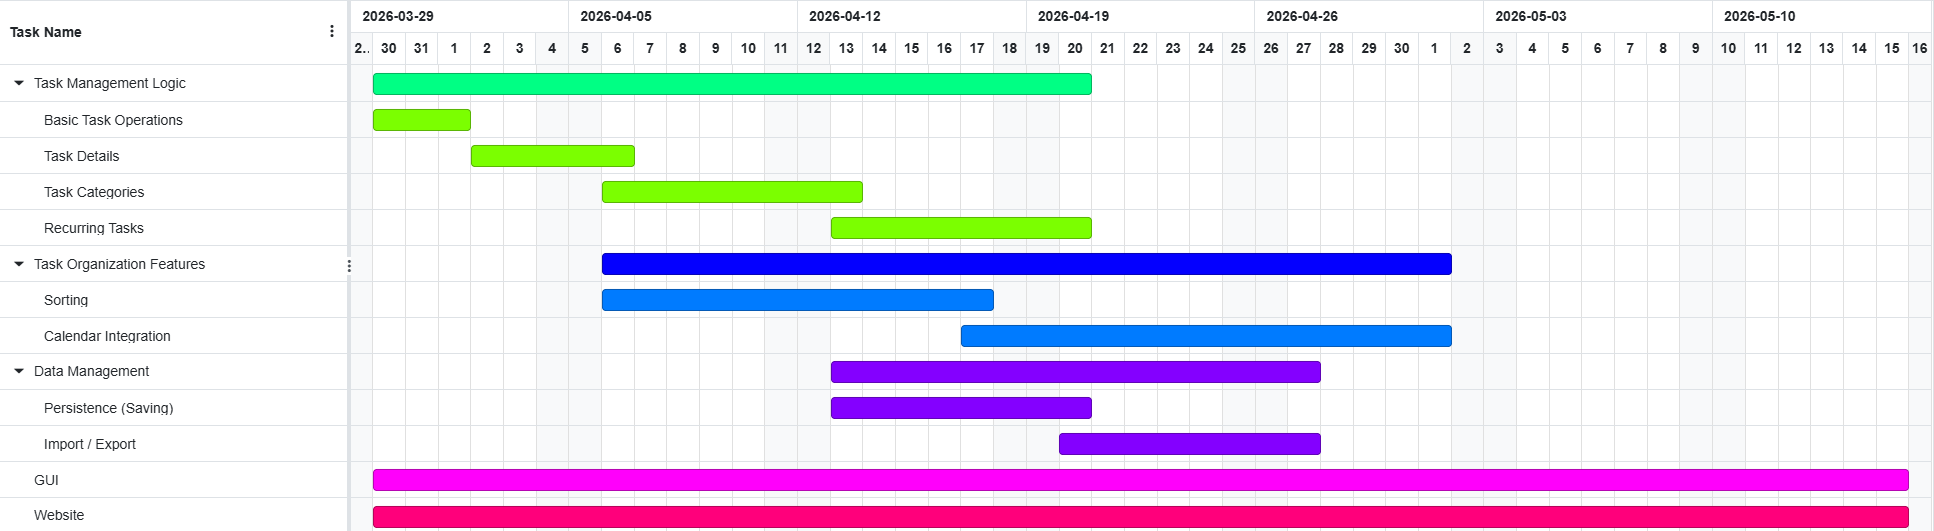
\includegraphics[width=9in, angle=90]{gantt_chart/gantt_diagram.png}
\end{figure}

\end{document}